\documentclass[paper=a4, fontsize=11pt]{jhwhw} % A4 paper and 11pt font size
\usepackage{amsmath,amsfonts,amsthm, amssymb} % Math packages
\setlength\parindent{0pt} % Removes all indentation from paragraphs - comment this line for an assignment with lots of text
\usepackage{graphicx}
\usepackage{verbatim}
\usepackage{enumerate}
\usepackage{mathtools}
\usepackage{color}
\newcommand\SetSymbol[1][]{\:#1\vert\:}
\providecommand\given{} % to make it exist
\DeclarePairedDelimiterX\Set[1]\{\}{\renewcommand\given{\SetSymbol[\delimsize]}#1}
\usepackage{listings}

\definecolor{dkgreen}{rgb}{0,0.6,0}
\definecolor{gray}{rgb}{0.5,0.5,0.5}
\definecolor{mauve}{rgb}{0.58,0,0.82}

\lstset{frame=tb,
    language=Java,
    aboveskip=3mm,
    belowskip=3mm,
    showstringspaces=false,
    columns=flexible,
    basicstyle={\small\ttfamily},
    numbers=none,
    numberstyle=\tiny\color{gray},
    keywordstyle=\color{blue},
    commentstyle=\color{dkgreen},
    stringstyle=\color{mauve},
    breaklines=true,
    breakatwhitespace=true,
    tabsize=3
}



\begin{document}
\title{MP1}
\author{Ben Haines}

\section{Part 1}
\subsection{Normalization Implementation}
\begin{lstlisting}
public String Normalization(String token) {
    // remove all English punctuation
    token = token.replaceAll("\\p{Punct}+", "");
    // convert to lower case
    token = token.toLowerCase();

    //Note that this doesn't attempt to recognize doubles
    //This is because all periods were removed in the previous step.
    //At this point in the processing a double looks the same as an int.
    token = token.replaceAll("\\d+", "NUM");

    return token;
}
\end{lstlisting}

\subsection{Graphs}
\begin{figure}[h!]
    \caption{Total Term Frequency}
    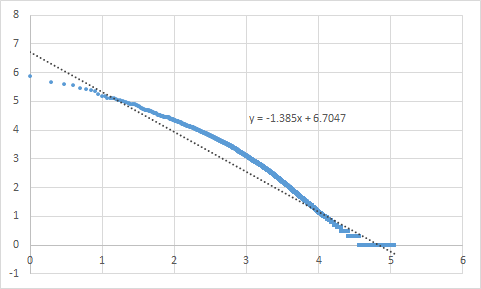
\includegraphics{ttfoutgraph}
\end{figure}
The y-axis on the above graph is total term frequency. The x-axis is rank of the word by total term frequency. Both axes are log scaled.

\begin{figure}[h!]
    \caption{Document Frequency}
    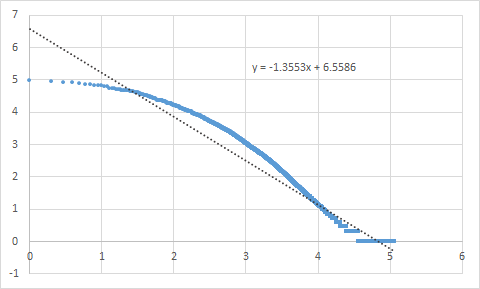
\includegraphics{dfoutgraph}
\end{figure}
The y-axis on the above graph is document frequency. The x-axis is rank of the word by document frequency. Both axes are log scaled.
\subsection{Questions}
From looking at the graphs above there appears to be a strong linear fit. The $R^2$ scores of 0.8981 for the document frequency curve and 0.9026 for the term frequency curve confirm that the data is fit well by a linear model and that total term frequency fits Zipf's law slightly better on this set. From inspecting the graph it seems that the better fit is mostly explained by the high rank words. On the document frequency graph the high ranking words are not as frequent as the model predicts. One possible explanation for why this might be is that there are certain words that would be expected to be used with high frequency in restaurant reviews, such as "wait" and "deliver", but which are limited to a subset of the actual documents. The word deliver might be used frequently but its document frequency is limited to the subset of reviews about locations that offer delivery. The data somewhat supports this idea as "deliveri" has rank 1454 by total term frequency but is over a hundred spots lower at 1568 when ranked by document frequency.  

\section{Part 2}
\subsection{Restaurant Specific Stopwords}
It was unclear to me at what point in the process we were intended to remove stopwords. My interpretation of the instructions was that we should find the top hundred N-grams in the Yelp data set and from these remove the stopwords that already appeared in the generic stopwords list. This left me with the following 33 N-grams with the highest document frequency that were not located in the generic stopwords list. For each N-gram their document frequency in the Yelp corpus is listed to the right. 
\begin{verbatim}
nt,48297.0
good,46806.0
food,46168.0
NUM,44920.0
great,34293.0
it was,31916.0
and the,31817.0
of the,31642.0
order,31258.0
time,30737.0
wait,28864.0
this place,27228.0
it s,25850.0
servic,25566.0
back,24607.0
in the,24114.0
friend,23540.0
the food,22934.0
love,22773.0
on the,22547.0
and i,22507.0
ve,20605.0
delici,20242.0
do nt,19840.0
i was,19625.0
restaur,19431.0
if you,19136.0
for the,19025.0
fri,18998.0
for a,18885.0
eat,18829.0
\end{verbatim}

It's interesting to see what things are specific to the Yelp review corpus. Some of the words are predictable results of properties of the dataset. Things like "good", "food", "eat", "delici", and "restaur" make sense in the context of restaurant reviews. Other terms seem to be a result of the particular way the data was processed rather than any characteristic of the data itself. The 2-grams "i was", "and i", and "on the" are simply combinations of two stopwords. Later when I filter stopwords out of the vocabulary I check if either token in a given 2-gram is a stopword and remove it if it is. This means that the addition of things like "i was" and "and i" to the stopword list is redundant and doesn't provide any extra filtering. Other terms like "nt" and "ve" seem to tell us something about the tokenizing process. The only reasonable source of these tokens that I can determine is from contractions like "they've", "didn't", and so on. It's interesting that these are separated into separate tokens, 

"NUM" is another interesting case that results from the method of processing. It makes sense that numbers should be common in the context of restaurant reviews. They could come up in things like price, the amount of time spent waiting for service, or the number of options on the menu. Obviously "NUM" as a string is not very common in english text so this is a good example of how merging the retaurant stopwords and the generic stopwords provides extra utility. 

\subsection{Size of Vocabulary}
The final size of my controlled vocabulary was 7385 uniqe N-grams. 

I thought that this number was surprisingly low. Considering that there were over a hundred thousand reviews, each presumably a few sentences long, I was expecting there to be a similarly large resulting vocabulary. Part of the reason the vocabulary is so small is a result of my aggressive stopword filtering method mentioned above. A less aggressive approach would be to only filter out 2-grams for which each individual token is a stopword rather than filtering all 2-grams where either token is a stopword. It would be interesting to compare the results of the two approaches. Filtering fewer N-grams from the vocabulary would on the one hand decrease the specificity of the information known about each document but on the other hand might include useful information to assist in making similarity measures. 

\subsection{Top \& Bottom Fifty}
The top fifty N-grams from the controlled vocabulary and their corresponding inverse document frequency scores were:
\begin{verbatim}
tabl,2.7116603133011816
make,2.737570204894965
sauc,2.7613178742505755
dish,2.8247939379762204
tast,2.829477217527197
menu,2.8641505826978757
amaz,2.8681347776915507
peopl,2.88661770080504
thing,2.8934184653823047
pretti,2.9231001061293904
seat,2.9310313212495043
night,2.9354272299954354
nice,2.9502443390133584
drink,2.980553921747443
chees,2.9826123389131887
worth,3.036474317009053
meal,3.056698448842647
flavor,3.072197853080766
bar,3.0766372855832493
perfect,3.0852607319353638
recommend,3.113690339660403
price,3.1143385853682184
experi,3.1518326551496565
chicken,3.1535171497785797
dinner,3.163003119105742
bit,3.1694060094656775
star,3.1812955266228484
made,3.1858996263164845
long,3.188427852239256
enjoy,3.2401071370186005
side,3.2498984585454904
pizza,3.250362689555174
top,3.254457242083833
favorit,3.2561371304863562
small,3.263073141046602
serv,3.289085755381581
hour,3.290728188483516
lot,3.3013236703529274
review,3.3035738302809716
day,3.308581450348138
minut,3.3098619233130475
beer,3.3298715501516107
ll,3.3354173168229253
line,3.3540941877274566
fresh,3.395530188918025
expect,3.4041574396670553
chicago,3.4061088713357592
big,3.4188868533097336
ca,3.4323871136772057
feel,3.4534405228750376
\end{verbatim}

The bottom fifty N-grams from the controlled vocabulary and their corresponding inverse document frequency scores were:
\begin{verbatim}
NUMfood,8.622673736011537
dinela,8.622673736011537
alltim favorit,8.622673736011537
thirst,8.62267373601153
primari,8.622673736011537
chicken tender,8.622673736011537
top choic,8.622673736011537
left stuf,8.622673736011537
mislead,8.622673736011537
inlaw,8.622673736011537
west loop,8.622673736011537
waaay,8.622673736011537
eye roll,8.622673736011537
demolish,8.622673736011537
costilla,8.622673736011537
applaud,8.622673736011537
bit earli,8.622673736011537
memor meal,8.622673736011537
strawberri jam,8.622673736011537
contend,8.622673736011537
util,8.622673736011537
creativ dish,8.622673736011537
drama,8.622673736011537
big bowl,8.622673736011537
scan,8.622673736011537
brûlée,8.622673736011537
snap pea,8.622673736011537
teriyaki mayo,8.622673736011537
besti,8.622673736011537
outi,8.622673736011537
favorit dessert,8.622673736011537
egg potato,8.622673736011537
lifechang,8.622673736011537
marzano tomato,8.622673736011537
chees melt,8.622673736011537
NUMlb,8.622673736011537
browni cooki,8.622673736011537
tecat,8.622673736011537
super fun,8.622673736011537
unseason,8.622673736011537
chicken parm,8.622673736011537
nice sweet,8.622673736011537
herd,8.622673736011537
flap,8.622673736011537
eggi,8.622673736011537
dome,8.622673736011537
goulash,8.622673736011537
berkshir pork,8.622673736011537
meatloaf hash,8.622673736011537
perplex,8.622673736011537
\end{verbatim}

All of the bottom fifty (and more) N-grams in the controlled vocabulary had document frequency scores of 50 and thus identical inverse document frequency scores. 

\section{Part 3}
\subsection{Cosine Similarity Function}
\begin{lstlisting}
public double similiarity(Post p) {
    double magA = 0;
    double magB = 0;

    for (double i : idToTF_IDF.values()) {
        magA += Math.pow(i, 2);
    }

    for (double i : p.idToTF_IDF.values()) {
        magB += Math.pow(i, 2);
    }

    magA = Math.sqrt(magA);
    magB = Math.sqrt(magB);
    double denom = magA * magB;
    double numer = 0;

    //Get IDs of N-grams that are in both documents
    HashSet<Integer> intersection = new HashSet<Integer>(idToTF_IDF.keySet()); // use the copy constructor
    intersection.retainAll(p.idToTF_IDF.keySet());

    for (Integer i : intersection) {
        numer += idToTF_IDF.get(i) * p.idToTF_IDF.get(i);
    }

    return numer/denom;
}
\end{lstlisting}

The above similarity function is implemented as a method of the provided Post class. In my implementation each N-gram in the vocabulary is assigned a unique ID number. The instance variable 'idToTF' is a hashmap that maps the IDs of all of the N-grams contained in the particular document to the TF-IDF score of that N-gram in that document. 

\subsection{Most Similar Results}
\begin{itemize}
    \item Query 0
        \begin{enumerate}
            \item Score: 0.25522894822512215\\
                Author: G M.\\
                Date: 2012-10-02\\
                Content: no delivery????????????????????????????please!!!!!
            \item Score: 0.2493054844121245\\
                Author: David W.\\
                Date: 2011-11-12\\
                Content: I took a group of 12 friends there based on the recommendation of a friend.... It was some of the blandest Thai food I have ever had. The Panag Nua was tough and lacking in flavor. It was a true Panag curry but it just seemed watered down. The meat had been just sliced and tossed in. Normally good Thai places have nice chunks of beef that they let stew in it all day so the sauce permeates it and the meat just falls apart. The Yum Yai salad had almost no sauce and what litte sauce it did have lacked in any flavor.The Tom Ka Guy soup was watery and heavily lacking in taste. The chicken in it was dry and huge chunks that were just not right for a soup. It also lacked a decent amount of mushrooms.The Kow Pat Moo was totally flavorless for a Thai fried rice. It was more like over priced panda express Chinese fast food rice.  This is a huge failure. I mean how hard is it to toss nam plaud and sugar into some rice? The Phad Thai was soggy and had more the consistency of spagetti with marinara then a thai fried noodle dish. The saving grace was the moo sautee. It was nice and small like you would get on the streets of bangkok. It did taste good but then again that's the staple of Thai places and you would have to go out of your way to screw this one up.All this being said my friends liked it BUT none of them have ever tried Thai food before much less GOOD Thai food. I think this must be the case for a lot of the positive reviews here. An other negative reviewer pointed out that there simply no Thai people in there this does tend to be a good indicator as to if a Thai place is good.
            \item Score: 0.2486666214472175\\
                Author: Rebecca H.\\
                Date: 2013-04-14\\
                Content: Interesting flavors, delivery was very quick. 3.5
        \end{enumerate}
    \item Query 1
        \begin{enumerate}
            \item Score: 0.342130834046929\\
                Author: Homer S.\\
                Date: 2011-08-29\\
                Content: ok, i've now been to Avec a few times \& feel very confident in giving them a very well deserved 5 stars.for the service.it was impeccable. our waiter on Saturday was Marcus. he did a fantastic job overall, was also very friendly \& knowledgeable and gave the experience a very personal feel like if you were old friends (\& yet still professional),timing of everything was great, you'd not guess it was a busy saturday night.and for the food..first off we had the chorizo stuffed, bacon wrapped dates \& a marinated kale salad with turnips. Both were fantastic but the dates will always be the first thing i order. as soon as i sit down, every time i go here. they are ridiculous.the dates are sitting in a tomato sauce that's fantastic as well, we were spreading it not only on the fresh bread that comes with the dates but on the foccachia we got later as well, very good. i feel sorry for the cooks who prep the dates, as i imagine they probably have to make enough for at least one dish for every table that sits down, every single night.  (thank you chefs, i promise you it is appreciated.)next up we had foccachia stuffed with tellagio, ricotta, truffle oil \& herbs.this too was amazing. finally with our coffees we had some nice tempered chocolate crisps with something in the middle that they described as like crepes. we also had a) white chocolate panna cotta with figs \& apricot i think? i felt the panna cotta had a very good texture \& flavor but may have been a touch sweet for my taste, i will say, however, that if i'd ordered another coffee to accompany the panna cotta i would have enjoyed it a lot more with the contrasting flavors.all in all, even though we weren't hungry enough to eat a ton of food, this was easily one of the best dinners i've had in a long time. I can't wait to go back.
            \item Score: 0.3006593167010708\\
                Author: Sonya T.\\
                Date: 2012-05-27\\
                Content: Food is pretty good here. We had several small plates; most notably recommend the squid. Had also had the roasted chicken and pork shoulder, both were also very good. The panna cotta was simply delicious. Still not crazy about the communal seating like the owner's other restaurant, the publican.
            \item Score: 0.3000856915721334\\
                Author: Shyamala L.\\
                Date: 2013-08-25\\
                Content: A must-visit if you are in Seattle for any duration of time. I cannot have enough of their  pizzas - the crust is unbelievably light and airy, and the toppings are just perfect. Kudos to them for having an equal balance of veggie \& meat options. Try their Panna Cotta, and see if that does not keep you coming back for more.
        \end{enumerate}
    \item Query 2
        \begin{enumerate}
            \item Score: 0.2677818275494673\\
                Author: Bo Y.\\
                Date: 2013-08-21\\
                Content: Good food! Fast!Ordered chicken taco and "taco on the walk" Very tasty.Cash only
            \item Score: 0.2758902277993126\\
                Author: Benjamin D.\\
                Date: 2011-05-05\\
                Content: Holy pork belly tacos!
            \item Score: 0.2975138902006175\\
                Author: Rory B.\\
                Date: 2009-11-12\\
                Content: Best. Tacos. Ever.
        \end{enumerate}
    \item Query 3
        \begin{enumerate}
            \item Score: 0.2555649806227921\\
                Author: Amy W.\\
                Date: 2010-02-24\\
                Content: Gosh, my review before was short.  It's okay, I can make it up now.  They close between lunch and dinner, so don't come here in the middle of the day. Upon entering the small parking lot, you will need to grab a ticket from the machine.  Don't forget to validate it before you leave, so your parking fee will only be \$2.50.  There's metered parking on the street as well, but sometimes it's tough to find a good spot.We got here around 5:15 on a Monday night.  They open at 5:30 for dinner, and already there were 7 parties before us waiting.  We were still sat right away though.  Looking around the room, most people order the sashimi or sushi set dinners, since they are great deals.  Since I'm cutting back on eating raw fish, yes I know it sucks, I ordered a few cooked appetizer dishes.For sure one of the great things about their menu is that it does cater to everyone.  They have the more "americanized" items like beef or chicken teriyaki bento to the izakaya style tapas to fresh sashimi and sushi.I ordered the Salmon skin salad, Ankimo (monkfish liver), Ume-Shio cut roll and Grilled Yellowtail collar.  My dinner-mates all ordered the sashimi dinner.  We also ordered Uni sashimi for the table to share.Salmon skin salad was just okay.  Nothing to rave about.  Actually I barely had an salmon skin.  Ankimo was delicious and fresh!  By the way, ankimo is not a raw dish.  It's steamed, but served cold.  Ume-shiso cut roll was not the best I've had.  It was more salty than sour.  Ikko actually makes the best ume-shiso cut roll.  The yellowtail collar was grilled perfectly and just super tasty!  The portion was also rather large too!  I couldn't even finish it, had to share.  The uni was super duper fresh!  When ordering sashimi, they give you the whole box plus a side of chopped fatty tuna.  It's all accompanied with sliced cucumbers and crispy seaweed.  It's \$30, but so worth it.The sashimi dinner was a ridiculously large portion!  All for only \$26!  You get two small starts of pickled cucumber and a sunomono.  Then you get a big bowl of rice and a plate of mixed tempura.  Finally a full plate of fresh assorted sashimi.  My dinner mates were very satisfied and full.  The servers were also very nice and filled our hot teas regularly.  Oh, they have lots of ice creams and mochi ice creams for dessert as well as exotic fresh fruits such as cherimoya.  Definitely a great place to go for fresh and delicious Japanese for a good price!
            \item Score: 0.22874504168191584\\
                Author: Lawrence C.\\
                Date: 2011-06-04\\
                Content: This has been a long time coming, really.  In actuality, it's a travesty I didn't review this restaurant first.  This, to me, is the penultimate experience in sushi in the greater los angeles area.  I don't mean just in little Tokyo, I mean in the entire LA county.  While I can't claim to have tried every top flight sushi restaurant (urasawa is gonna be for a special occasion in the future), I have been eating sushi for 15+ years, up and down California, and without a doubt, sushi gen is my go to spot.  When someone asks me what I feel like eating at any given time, its sushi gen.  I have brought all of my friends that visit me to this wonderful establishment, and they all tell me I have excellent taste in food.  I wish I could take the credit, but to not like sushi gen must mean your taste buds must be allergic to excellence.You have the option of either eating at the bar (omakase style only, minimum of 4 orders per person) or at the tables.  When I come here, usually in small parties (between 2-5 people), I go for the table.  My go to meal?  The sashimi dinner with a side of tempura (\$26).  I think 95\% of the time I have dined at the table, I get that.   All the dinner plates start with miso soup, tsunemono, and pickled vegetables (usually a cucumber and cabbage concoction).  Lets start with the miso soup.  I feel like you can judge a good sushi restaurant by the attention to detail in the miso soup, having the correct ratio of dashi to miso paste, as well as having the tofu be unbroken.  Sushi gen hits all three of these aspects wonderfully; this is how I know this is the precursor to a wonderful meal.  The tsunemono is deliciously sweet and tart at the same time, serving to counterbalance the saltiness of the pickled vegetables and miso soup.  The salty pickled vegetables are the weakest part of the trio, but it's refreshing when eaten in conjunction with the other two items.After that comes the main course: a plate full of sashimi, a bowl of perfectly cooked hot sushi rice, and a side of shrimp and vegetable tempura.  The tempura itself is delicious; not too heavy, crispy, crunchy, and piping hot.  It's the perfect side to a cold plate of heavenly sashimi.  The usual suspects in an order of the sashimi dinner?  3 slices of tuna (sometimes fattier, sometimes leaner), 3 slices of hamachi, their house special spicy tuna (I guarantee you its like no other spicy tuna you've ever had), chunks of yellowtail, chunks of regular tuna, tamago, either tako or ikura (octopus or squid), some sweet preserved fish (this is indistinguishable to me), and a cooked piece of salmon (kind of the odd man out), all served with a generous helping of seaweed.  The specifics are up to the sushi chefs, but it usually comes out like that in some fashion.  All of the fish is of the highest quality, although I wish they served salmon sashimi instead of the cooked salmon (they don't make substitutions).  A comparable plate would cost 3-4 times as much at any other establishment west of downtown (sasabune and hide sushi come to mind, but I'll be honest, those restaurants pale in comparison), and the portions are so generous it borders on the obscene.  For my money, the sashimi dinner combo is the best meal in town, and I will challenge you to a duel if you dare dispute this.I've also had the pleasure of trying their various appetizers, from the ankimo to their fried chicken, and the quality of the food is definitely there.  But honestly, if you are going to go to a sushi restaurant in the heart of Little Tokyo, you should be eating the raw goods and eschew the cooked.I've only eaten the omakase once before, but I must say, it was absolutely delightful.  While I am sure there are better authorities than I to the world of omakase, the flavour pairings and the order of the fish prepared by the chef were simply superb.  From what I recall, we started with the prototypical orders of fish, including toro, hamachi, and mackerel.  It pains me to say it, but the quality of the fish served with the omakase is just out of this world, just a cut above what is offered to the main restaurant.  Pun intended.  We proceeded with other more adventurous fare: albacore with thinly sliced green onions, mirugai with a touch of yuzu pepper for added kick, and scallops so sweet it threatens to overwhelm.  A nice touch is that the chef intersperses the orders in a way where some of the nigiri you eat with soy sauce, and some you don't; he will tell you beforehand what the proper way of eating the order is.  The amaebi is also exceptionally sweet, with the fried head serving as a textural counterpoint to the sweet shrimp.  The only downside to the omakase?  It can easily run you 50+ per person before sake, which ups the joint a dollar sign.  It's a bit more decadent than the table meal, but either way, you can't go wrong with Sushi Gen.
            \item Score: 0.2108206734495474\\
                Author: Alissar T.\\
                Date: 2013-04-28\\
                Content: Insanely trendy, sleek and sexy, a night at Buddakan is a special one. The service is attentive, the drinks are incredible and the food is surprisingly good for a place so 'scene-y'. Usually at a place with this much hype and an atmosphere so gorgeous (the main dining room was where Carrie's rehearsal dinner in Sex and the City was filmed), you expect to pay mainly for the atmosphere and perhaps a good cocktail. However Buddakan has perfected all three important categories: atmosphere, cocktails and food. The cocktails are as delicious as their alluring names appear to be. I chose the 'Dream', served with Bacardi Limon, Shochu (a Japanese alcohol), guava and mint. Upon first sip, I was envisioning the next time, and time after that I would be back to Buddakan to try all of their cocktails ('Tranquility'...'Reflection'...'Fever'). Yup. I'll be back for you.For appetizers, the Edamame Dumplings are essential. This appetizer alone is reason to come back to Buddakan. The dumplings are soft and delicate, and stuffed with an edamame filling enhanced with cream, dashi broth and truffle oil. It yields for a flavor and texture so luxurious, stuffed into dumpling dough so light and perfect. The dumplings are then cooked in a shallot and sauternes broth, with chicken stock, thyme and served with onion sprouts. Incredible! Bravo Chef Michael Schulson. I love you for this appetizer. The Sesame Shrimp Toast served with soy sauce and spicy mustard was also good; crispy and crunchy and coated with white and black sesame seeds and bursting with flavors of fresh shrimp. We also shared the Charred Asparagus with black bean foam, Lobster Fried Rice with saffron and thai basil, and the Roast Duck Noodles with duck wontons and sliced duck. The Charred Asparagus was simple yet amazing. I enjoyed the Lobster Fried Rice and the Roast Duck Noodles were delicious (from the duck meat to the wontons to the broth) but was a tad over-salted. We were so full  when it came time for dessert but the Crying Chocolate dessert was calling my name (and looked incredible on our neighbor's table)... Malted chocolate ganache, milk caramel, and Vietnamese coffee ice cream. Save room for dessert.Overall consensus: Buddakan rocks. It is a great place for a post-work drink and appetizers, place to take a friend from out-of-town, a birthday, or to impress your parents. I would recommend to stick mainly with the appetizers and lots o' cocktails.Other menu highlights I can't wait to try:Cantonese Spring Rolls with shrimp and chicken   Lobster Egg Rolls with mint, cabbage, and a sweet chili sauce  Hoisin Glazed Pork Belly with spicy shallots, cabbage, steamed 'buns'  Tuna Tartare Spring Roll with crispy shallots and ponzu  Crispy Calamari Salad with green apples, cashews, and miso vinaigrette Chili Rock Shrimp with toasted gingerBoneless Spare Ribs with chinese mustardMao Poe Tofu with minced pork and red chiliWhole Crispy Fish with chive blossom, green curry, and turmeric
        \end{enumerate}
    \item Query 4
        \begin{enumerate}
            \item Score: 1.0
                Author: Yaseman K.\\
                Date: 2014-05-22\\
                Content: I usually come here on friday or saturday nights with my friends, and its really crowded. Its a really cool atmosphere and we love coming here. Their pizzas and sweet potato fries are delicious! I love their food, its really good and theres a lot to choose from. Their desserts are definitely worth trying. Peach cobbler is a must!
            \item Score: 0.4451022596356447 \\
                Author: Erica I.\\
                Date: 2011-12-03\\
                Content: The mac and cheese and peach cobbler were the BEST!  I'd go back just for those.
            \item Score: 0.43383847264071934\\
                Author: Steve F.\\
                Date: 2013-06-09\\
                Content: Best ribs in ChicagoBaby backs are the best, try the peach cobbler if you have room.
        \end{enumerate}
\end{itemize}

\subsection{Inferences about Queries}
Judging only from the contents of the returned results it seems likely that we would be able to make informed guesses about what type of restaurant the original queries were reviewing. For query 0 two of the returned reviews mentioned delivery. This makes me think either pizza or Chinese. The longer third result is clearly describing a Thai restaurant. Based on this I would guess the original review was of either a Chinese or Thai restaurant. 

The results for query 1 mention pizza, panna cotta, and focaccia. I would be confident in guessing the original review was about an Italian restaurant. The results for query 2 are even more consistent. They are all about tacos. The original review in this case was likely about a taqueria.

Mentions of izakaya, sushi, and edamame dumplings suggest that query 4 was about a Japanese restaurant. 

For the final query one of the results had a cosine similarity of 1 with the query. This means that the contents of the review were identical. Because the review itself is fairly long and was unlikely to be duplicated by chance this probably means the review is the exact same. We can say conclusively then that the restaurant serves peach cobbler, pizza, and sweet potato fries. Based on the contents of the other reviews it is probably a classic American restaurant. 


Beyond the type of restaurant it would be interesting to see what other types of things might be inferred from the results of queries. For each of the examples here the results of a particular query all seem to indicate a similar level of positiveness about the restaurant being reviewd. Query 0 is the only one that returned any negative sounding reviews and it returned two of them, with the third being neutral. This suggests it might also be able to predict the rating given by the query review based on the returned results.
\end{document}

